\section{System Description} Havven is a dual-token system that, combined with a set of novel incentive mechanisms, stabilises the price of the nomin with respect to an external asset. Users of the nomin token pay the owners of the havven token for collateralising and stabilising the system. \\

\noindent The havven token incentivises those who hold it to fulfil two functions:

\begin{itemize}
\item{To provide the system with collateral.}
\item{To participate in the stabilisation of the nomin price.} \\
\end{itemize}

\noindent \textbf{Collateralisation} \\

\noindent Confidence in the stability of the nomin begins with overcollateralisation, so that the value of escrowed havvens is greater than the value of nomins in circulation. As long as the ratio of total nomin value to total havven value remains favourable, there is sufficient backing in the underlying collateral pool to ensure that nomins
can be redeemed for their face value. The redeemability of a nomin for the havvens against which it was issued strongly supports a stable price. \\

\noindent \textbf{Stabilisation Incentives} \\

\noindent Havven rewards those that have issued nomins. These rewards are derived from transaction fees and are distributed in proportion with how well each issuer maintains the correct nomin supply. The system monitors the nomin price, and responds by adjusting its targeted global supply, which individual issuers are incentivised to move towards. \\

\noindent Where volatility persists, stronger stabilisation mechanisms may be applied, for example automated collateral recovery. Where a significant portion of nomins are being used for hedging, (and hence not generating transaction fees) a charge can be applied to ensure that the cost of utility for hedging is not being solely borne by transactions.

\newpage

\subsection{Equilibrium Nomin Price}

\noindent We first introduce the core system variables:

\begin{align*}
H &\text{: havven quantity} & N &\text{: nomin quantity} \\
P_h &\text{: havven price}  & P_n &\text{: nomin price} \\
\end{align*}

% \todo[inline]{Consider renaming havven price symbol to reflect that it is computed from income}

\noindent All havven tokens are created at initialisation, so $H$ is constant.
The quantity of nomins floats, responding to the issuance actions of havven holders.
The Havven system needs to incentivise issuers to maintain $N$ such that
the nomin price $P_n$, is stable at \$1. As we proceed, we may subscript variables with $t$ to indicate the value of that variable at a given time. \\

\noindent In Havven, the measure of the value of nomins against the value
of havvens is called the collateralisation ratio:

\begin{equation}
C = \frac{P_n \cdot N}{P_h \cdot H} \label{eq:collateralisation}
\end{equation}

\vspace{3 mm}

\noindent From the law of supply and demand, there exists some supply
of nomins $N_{opt}$, where the related level of demand yields an equilibrium
price of \$1. This quantity is associated with an optimal collaterisation ratio
$C_{opt}$. We visualise this equilibrium below with a hypothetical demand and supply curve.  \\

% \todo[inline]{curved lines}
% \todo[inline]{make diagrams pretty}
\begin{center}
\begin{tikzpicture}[scale=3]

% draw axes
\draw [<->, thick] (0,2) node (yaxis) [above] {$P_n$} |- (2.5,0) node (xaxis) [right] {$N$};

% draw intersecting lines
\draw (0.5, 0.5) coordinate (a_1) -- (2,1.8) coordinate (a_2) node[pos=0.0, left] {S};
\draw (0.5, 1.8) coordinate (b_1) -- (2,0.5) coordinate (b_2) node[pos=1.0, right] {D};

% calculate coordinate of intersection
\coordinate (c) at (intersection of a_1--a_2 and b_1--b_2);

\draw[dashed] (yaxis |- c) node [left] {$\$1$} -| (xaxis -| c) node[below] {$N_{opt} = \frac{C_{opt} \cdot P_h \cdot H}{P_n}$};

\end{tikzpicture}
\end{center}

\noindent The system is unable to influence the demand for nomins. We assume that some level of demand exists given the utility of nomins as a stable cryptocurrency. Although demand cannot be manipulated, the supply of nomins is controlled by havven holders, whose issuance incentives are in turn controlled by the system. It follows that as we require a fixed price $P_n = \$1 $ and are unable to control either $P_h$ or $H$, we must manipulate $C_{opt}$ such that $N = N_{opt}$ in order to satisfy our requirement.

\subsection{Issuance and Collateralisation} 

% \todo[inline]{separate wallets from accounts}

\noindent Havven's goal is to remain overcollateralised. In order to do so, the system defines a collaterisation target:

\begin{equation}
0 < C_{opt} < 1  \label{eq:target}
\end{equation}

\vspace{2 mm}

\noindent It is necessary at this point to distinguish, for an account $i$, between the nomins it contains $N_i$ (equity) and the nomins it has issued $\check{N_i}$ (debt). Note that globally, the $\sum_{i}N_i = \sum_{i}\check{N_i}$, as all nomins were issued by some account. However, a given account may have a balance different from its issuance debt. Hence we can define the collateralisation ratio for an individual account $i$ in terms of its issuance debt:

% \todo[inline]{Make sure this equity/debt language is not too security-like.}

\begin{equation}
C_i = \frac{P_n \cdot \check{N_i}}{P_h \cdot H_i}  \label{eq:individualcollateralisation}
\end{equation}

\vspace{2 mm}

\noindent The system provides incentives for individual issuers to bring their $C_i$ closer to $C_{opt}$ while maintaining $C_{opt}$ itself at a level that stabilises the price. \\

\noindent \textbf{Nomin Issuance} \\

\noindent The nomin issuance mechanism allows Havven to reach its collaterisation target.
Issuing nomins escrows some quantity of havvens, which cannot be moved until they are unescrowed.
The quantity of havvens $\check{H_i}$ locked in generating $\check{N_i}$ nomins is:

\begin{equation}
\check{H_i} = \frac{P_n \cdot \check{N_i}}{P_h \cdot C_{max}}  \label{eq:escrowed}
\end{equation}

\vspace{2 mm}

\noindent Under equilibrium conditions, there is some $\check{H_i} \leq H_i$ when $C_i = C_{opt}$, which the issuer is incentivised to target. These incentives are provided in the form of transaction fees, discussed in section 2.4. It is important to note that the issuer may voluntarily increase their $C_i$ up to the limit of $C_{max}$; for example if they anticipate a positive movement in $C_{opt}$. \\

\noindent On the other hand, an issuer may not issue a quantity of nomins that would lock more than $H_i$ havvens.  Consequently, $C_i$ may never exceed $C_{max}$, except by price fluctuations, and in such circumstances, issuers are rewarded for bringing $C_i$ back under $C_{max}$. \\

\newpage

\noindent After generating the nomins, the system places a \textbf{limit sell} order with a price of \$1 on a decentralised exchange. This means that the nomins will be sold at the current market price, down to a minimum price of \$1. If we assume implementation on Ethereum, then the nomins are sold for an equivalent value in ether, with the proceeds of the sale remitted to the issuer. \\

\noindent \textbf{Nomin Destruction}

\vspace{1mm}

\noindent In order to access the havvens that have been escrowed, the system must destroy the same number of nomins that were originally issued. When the issuer indicates the intention to retrieve their havvens, the system places a \textbf{limit buy} order on a decentralised exchange, up to a maximum price of \$1. The system places this order on behalf of the issuer and upon completion, the nomins are immediately destroyed. \\

\newpage
\subsection{Transaction Fees} Havven needs a direct incentive mechanism that can correct changes in the global collaterisation ratio, $C$, when the price of havvens or nomins changes. \\

\noindent Some of the equations below are defined in the discrete time domain and are referenced with a subscript $t$. These will be specifically used in our game theoretic modelling.

\subsubsection{Nomin Transaction Fees} Every time a nomin transaction occurs, the Havven system charges a small transaction fee. Transaction fees allow the system to generate revenue, which it can distribute to havven holders as an incentive to maintain nomin supply at $C_{opt}$. \\

\noindent The fee rate charged on nomin transactions is $\alpha_c$. It is constant and will be sufficiently small that it provides little to no friction for the user: \\

\begin{equation}
\alpha_c = k \ \label{eq:5}
\end{equation}

\begin{center}
\begin{tikzpicture}[scale=3]

% draw axes
\draw [<->, thick] (0,2) node (yaxis) [above] {$\alpha_c$} |- (2.5,0) node (xaxis) [right] {$P_n$};

% draw one line
\draw (0.0, 0.75) coordinate (a_1) -- (2.4,0.75) coordinate (a_2);

\coordinate (c) at (1.75, 0.75);

\draw[dashed] (yaxis |- c) node [left] {k};

\end{tikzpicture}
\end{center}

\noindent We may then express the total fees collected in period $t$, $F_t$, as a function
of the velocity of nomins $v_t$ and the total nomin supply $N_t$:

\begin{equation}
    F_t = v_t \cdot \alpha_c \cdot N_t
\end{equation}

\newpage
\subsubsection{Fees Received by Havven Holders}

\noindent The fee rate paid to a havven holder that has escrowed is $\alpha_r$.
The actual fee they receive is $\check{H_i} \cdot \alpha_r$, being proportional with the value they escrow.
This rate changes with respect their unique collaterilisation ratio, $C_i$. It increases linearly to a maximum $\alpha_{base}$ at the optimal collaterilisation ratio $C_{opt}$, before quickly
diminishing as $C_i$ approaches the maximum collaterisation ratio $C_{max}$.  \\

\noindent This function is designed to encourage havven holders to constantly
target the optimal collateralisation ratio, by rewarding them with greater
fees if they do so.\\


 % \todo[inline]{figure out whether t stays}

\begin{equation}
\alpha_{r,t,i} = \alpha_{base,t} \cdot \mathcal{F}_{i,t}(C_{i,t}, C_{opt}, C_{max,t})  \label{eq:feesreceived}
\end{equation}

\begin{equation}
\mathcal{F}_{i,t}(C_{i,t}, C_{opt,t}, C_{max,t}) = 
\begin{cases}
 \frac{C_{i,t}}{C_{opt,t}} &\mbox{when } C_{i,t} \leq C_{opt,t} \\[1em]
 \frac{C_{max,t} - C_{i,t}}{C_{max,t} - C_{opt,t}} &\mbox{when } C_{opt,t} \leq C_{i,t} \leq C_{max,t} \\[1em]
 0 &\mbox{otherwise}
 \end{cases}
 \label{eq:7}
\end{equation}

\begin{center}
\begin{tikzpicture}[scale=3]

% draw axes
\draw [<->, thick] (0,2) node (yaxis) [above] {$\alpha_r$} |- (2.5,0) node (xaxis) [right] {$C_i$};

% draw two lines
\draw (0.0, 0.0) coordinate (a_1) -- (1.75,0.75) coordinate (a_2);
\draw (1.75, 0.75) coordinate (a_1) -- (2.25,0.0) coordinate (a_2);

\coordinate (c) at (1.75, 0.75);
\coordinate (d) at (2.25, 0.0);
\coordinate (e) at (0.00, 0.00);

\draw[dashed] (yaxis |- c) node [left] {$\alpha_{base}$} -| (xaxis -| c) node[below] {$C_{opt}$};
\draw[dashed] (yaxis |- e) node [left] {$\alpha_{base}$} -| (xaxis -| d) node[below] {$C_{max}$};

\end{tikzpicture}
\end{center}

\noindent This fee distribution curve encourages havven holders who have escrowed to maintain their $C_i$ at $C_{opt}$.  \\

\newpage

\subsubsection{Base Fee Rate}

Let us define the total fees paid to havven holders $F_{r,t}$: \\

\begin{equation}
F_{r,t} = \sum_{i} \check{H_i} \cdot \alpha_{r,t,i} \label{eq:totalfeesreceived}
\end{equation} \\

\noindent Havven requires that the total fees collected from users has to be equal to the total amount of
fees paid to the havven holders, so that $F_{r,t} = F_t$. Substituting our earlier definition \eqref{eq:feesreceived} for $\alpha_{r,t,i}$ and solving for $\alpha_{base,t} $: \\

\begin{equation}
\alpha_{base,t} = \frac{F_t}{\sum_{i} \check{H_i} \cdot \mathcal{F}_{i,t}(C_{i,t}, C_{opt,t}, C_{max,t})} \label{eq:10}
\end{equation} \\

\noindent We have now defined the maximum fee rate, $\alpha_{base}$, in terms of the fees collected, $F_t$. This rate should be achieved when an individual's $C_i$ is at $C_{opt}$. \\

\noindent The definition of $C_{opt}$ must therefore provide the following incentive. If $P_n > \$1$ then the system must encourage more nomins to be issued. However, if $P_n < \$1$, the system must encourage nomins to be burned. 

\newpage

\subsection{Collateralisation Ratio}
\subsubsection{Optimal Collateralisation Ratio}

\noindent The optimal collaterilisation ratio $C_{opt}$ is a target for havven
holders to reach in order to maximise the amount of fees they receive.
$C_{opt}$ is defined in terms of the nomin price $P_n$, such that its value directly tracks changes in the nomin price; a havven
holder wishing to maximise their fees will target $C_{opt}$ by issuing or destroying nomins. \\

\noindent The function for $C_{opt}$ given below provides our dynamic target
for havven holders based on the price of nomins:

\begin{gather} \label{eq:optcollateralisation}
\begin{align}
\begin{split}
C_{opt,t} &= f(P_{n,t}) \cdot C_t  \\ 
f(P_{n,t}) &= max(\sigma \cdot (P_{n,t} - 1)^{\phi} + 1, 0) \\
\sigma & \text{: price sensitivity parameter } (\sigma > 0)\\
\phi   & \text{: flattening parameter } (\phi \in \mathbb{N} \text{, } \phi \nmid 2) \\
\end{split}
\end{align}
\end{gather}


\begin{center}
\begin{tikzpicture}[scale=1.15]
\begin{axis}[
    axis lines = left,
    xlabel = $P_n$,
    ylabel = {$f(P_n)$},
    xtick = {1},
    ytick = {0},
    y label style={at={(axis description cs:.15,1.00)}, rotate=270,anchor=south},
    x label style={at={(axis description cs:1.05,.13)},anchor=north},
]
\addplot[
domain=0:2,
range=0:2
]
{(x-1)^3 + 1};
\addplot [
domain=0:2,
range=0:2,
dashed
]  
 {x};
 \addplot[dashed, samples=50, smooth,domain=0:6] coordinates {(1,1)(1,0)};
\end{axis}
\end{tikzpicture}
\end{center}

\noindent When $P_n$ is at \$1, $C_{opt} = C$ and there is no incentive given to move away from the current global collateralisation level. However, if $P_n < \$1$, then $C_{opt} < C$, incentivising issuers to burn nomins, thereby raising the price. The $P_n > \$1$ case is symmetric. Notice that when the $P_n$ is close to \$1, $ f'(P_n) $ is small. However, the further it diverges from \$1, the larger the slope becomes, providing a stronger incentive, in the form of potential fees, for a havven holder to move toward $C_{opt}$. \\

\newpage

\subsubsection{Maximum Collateralisation Ratio}

\noindent Havven seeks to maintain $C \leq C_{opt} < C_{max} < 1$, in order to retain sufficient overcollateralisation. It might seem intuitive that $C_{max}$ should be a static value. However, since $C_{opt}$ varies linearly with $P_n$ and inversely with $P_h$,  there are situations where $C_{max}$ may need to change. Below we define $C_{max}$ in terms of $C_{opt}$. \\

\begin{gather} \label{eq:maxcollateralisation}
\begin{align}
\begin{split}
C_{max,t} &=  a \cdot C_{opt,t} \\ 
a & \geq 1 \\
\end{split}
\end{align}
\end{gather}

\begin{center}
\begin{tikzpicture}[scale=1.15]
\begin{axis}[
    axis lines = left,
    xlabel = $C_{opt}$,
    ylabel = {$C_{max}$},
    xtick = {1},
    ytick = {0},
    y label style={at={(axis description cs:.15,1.00)}, rotate=270,anchor=south},
    x label style={at={(axis description cs:1.08,.13)},anchor=north},
]
\addplot[
domain=0:1.00
]
{1.25 * x};
\addplot [
domain=0:1.00,
dashed
]  
 {x};
 \addplot[dashed, samples=50, smooth,domain=0:6] coordinates {(1,1)(1,0)};
\end{axis}
\end{tikzpicture}
\end{center}

\noindent The value of $C_{max}$ determines how overcollateralised each nomin is at issuance. The higher its value, the more nomins can be generated for the same quantity of havvens. In contrast, if $C_{max}$ is low, the system has a greater capacity to absorb negative shocks in the havven price before it becomes undercollateralised.  The value of $C_{max}$ therefore represents a tradeoff between \textit{efficiency} and \textit{resilience}. By defining $C_{max}$ as a function of $C_{opt}$, Havven finds the optimal balance in this dilemma. This ensures that like $C_{opt}$, $C_{max}$ only changes as a consequence of instability in the nomin price. \\

\noindent It should be noted that $C_{max} > 1$ corresponds to a fractional reserve monetary system, where a greater value of nomins can be issued against each havven. In Havven, this situation is unsustainable because it would cause simultaneous appreciation of havvens (up to at least the value of nomins issuable against a havven) and depreciation of nomins, immediately diminishing $C$, $C_{opt}$ and $C_{max}$, bringing them back under $1$.

\subsection{Issuance and Fees Example} 

\noindent Bob decides to purchase 100 havvens at \$1 each. Consider the following initial conditions:

\begin{align*}
C_{max} &= 0.5 & C_{opt} &= 0.4 & C &= 0.4 \\
P_n &= 1 & P_h &= 1 & H_i &= 100 \\
\sigma &= 50 & \phi &= 3 & a&= 1.25
\end{align*}

\noindent The system is in price equilibirum, with the global collateralisation ratio $C$ equal to the optimal collaterisation ratio $C_{opt}$. Initially,  Bob's wallet contains only free havvens.

\begin{figure}[h!]
\centering
    
\includegraphics[width=0.40\textwidth]{img/wallet}
\end{figure}

\noindent Bob wants to earn the maximum possible fees, so he issues nomins up to $C_{opt}$. The system generates 40 nomins and escrows 80 of his havvens, locking \$80 worth of value in the system. The nomins are sold for \$40 worth of ether and the proceeds are transferred to Bob's account.
\begin{figure}[h!]
\centering
    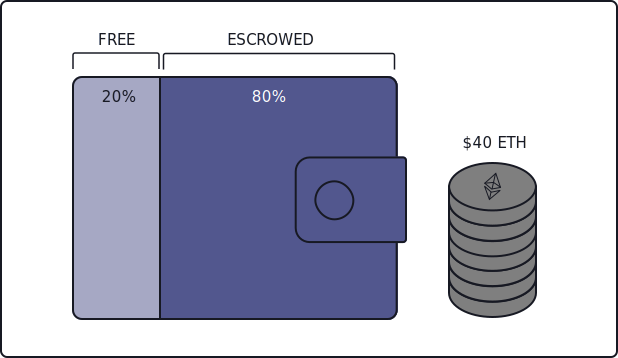
\includegraphics[width=0.6\textwidth]{img/escrowed}
\end{figure}

\noindent \textbf{Nomin Price Change} This example shows how the system incentivises havven holders to correct instability in the nomin price.

\begin{enumerate}
\item{As a consequence of reduced demand in decentralised trading markets, the nomin price $P_n$ drops to \$.90. The system needs to incentivise havven holders to reduce the supply of nomins so that the price returns to \$1.00.}
\item{First, consider that both $C$ and Bob's $C_i$ have decreased to 0.36. Since the nomin price has changed, $C_{opt}$ is recalculated to 0.342, which is smaller than both $C_i$ and $C$. Consequently, $C_{max}$ also changes to 0.4275. This increases the percentage of Bob's havvens that are locked.}
\begin{figure}[h!]
\centering
    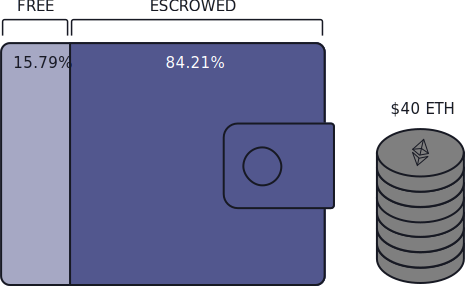
\includegraphics[width=0.6\textwidth]{img/pn_drop}
\end{figure}
\item{Bob now has a higher dollar value of locked havvens and his $C_i > C_{opt}$. This means that he is no longer receiving the maximum fee rate $\alpha_{base}$. In order to return to $\alpha_{base}$ he must lower his $C_i$ back to $C_{opt}$ by burning some nomins. He needs to work out how many to burn.}
\item{He should burn 2 nomins so that he has 38 total issued, which will cost \$1.80. When the system completes this process, his locked havvens will reduce back to 80. In addition, his $C_i$ is equal to $C_{opt}$ at 0.342, which means he is once again receiving the maximum fee rate.}
\begin{figure}[h!]
\centering
    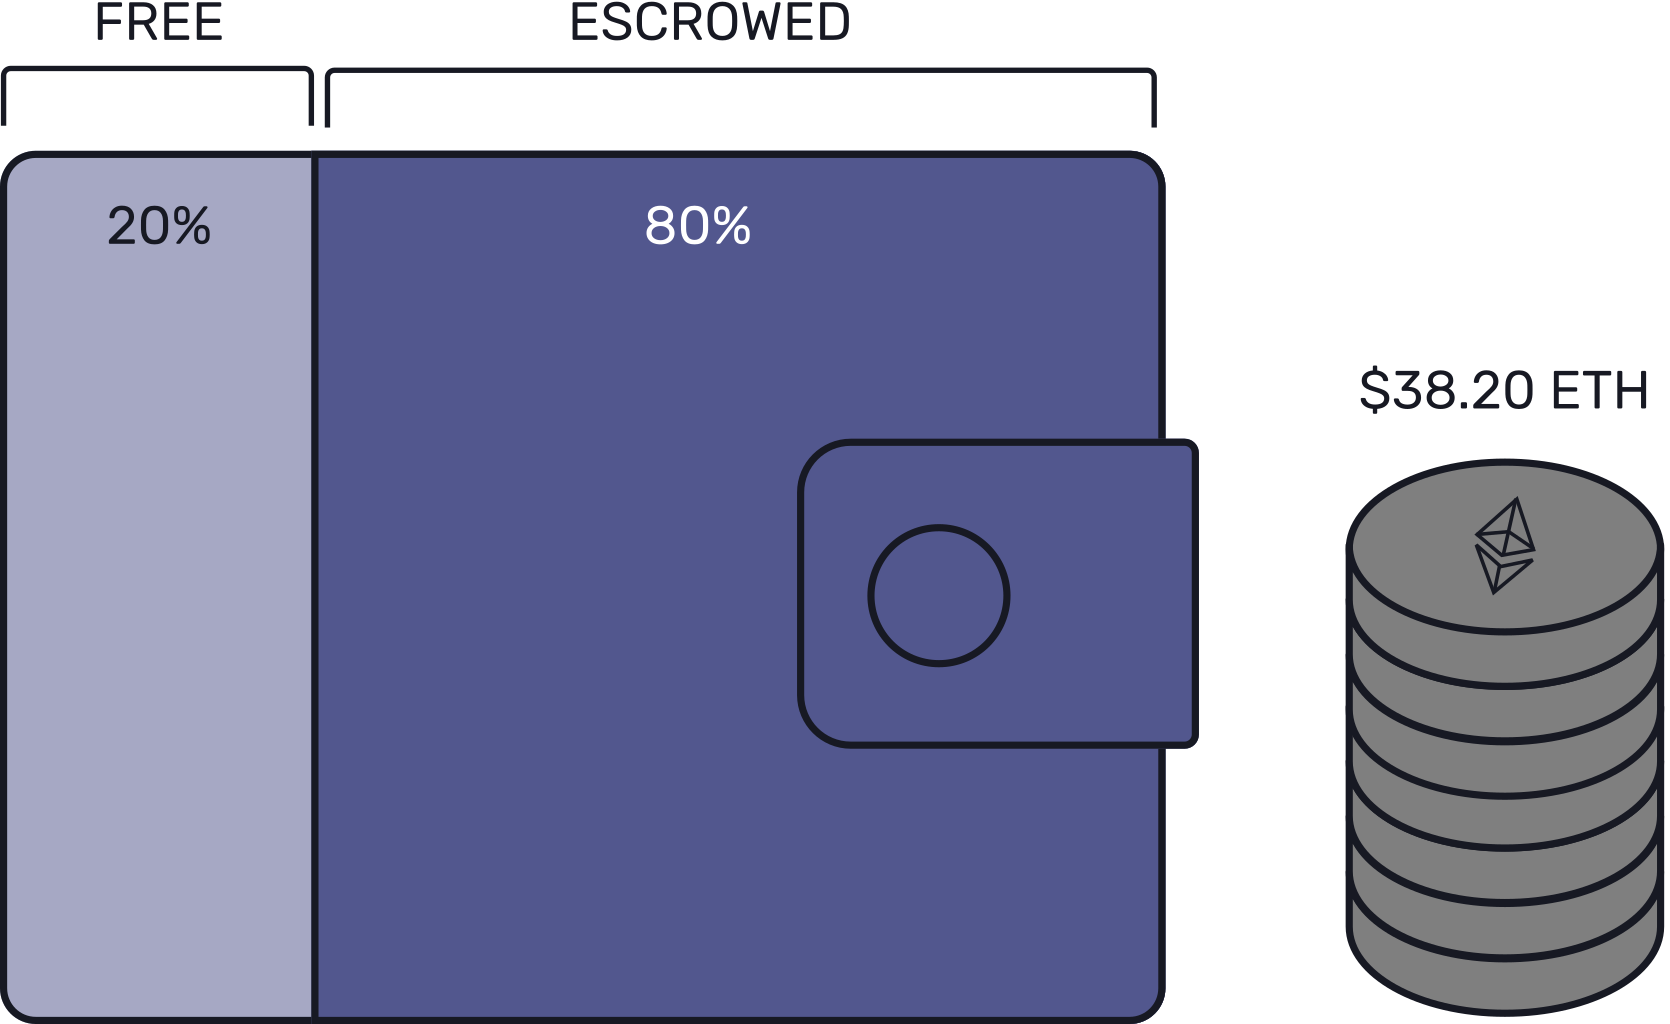
\includegraphics[width=0.6\textwidth]{img/post_burn}
\end{figure}
\item{Bob has taken the correct actions to raise the low nomin price. By electing to burn nomins, the system performed a limit buy order on his behalf, putting upward pressure on the nomin price. As compensation for doing so, he is rewarded with the optimal fee rate $\alpha_{base}$.}
\end{enumerate}

\newpage

\noindent \textbf{Havven Price Change (Market Price)} This example illustrates how the system maintains the dollar value of the underlying collateral by adjusting the quantity of a user's escrowed havvens when the havven price changes. Consider the same initial conditions as before:

\begin{align*}
C_{max} &= 0.5 & C_{opt} &= 0.4 & C &= 0.4 \\
P_n &= 1 & P_h &= 1 & H_i &= 100 \\
\sigma &= 50 & \phi &= 3 & a&= 1.25
\end{align*}

\begin{enumerate}
\item{Like before, Bob elects to issue up to $C_{opt}$ in order to maximise fees.}
\begin{figure}[h!]
    \centering
    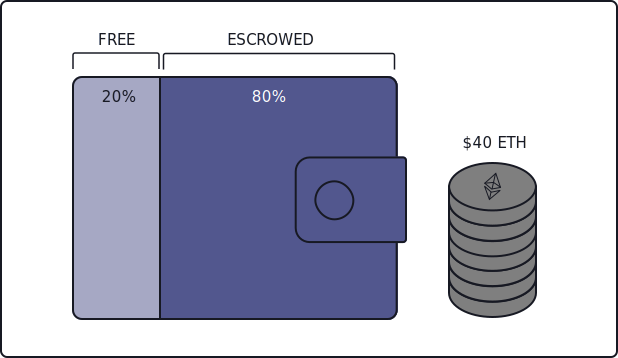
\includegraphics[width=0.6\textwidth]{img/escrowed}
\end{figure}
\item{The havven price $P_h$ drops to \$0.90, which means the value of Bob's wallet has decreased to \$90. Both $C$ and Bob's $C_i$ have increased to 0.44. Since the nomin price has not changed, the system does not need to incentivise issuance or burning. This is reflected in the new value of $C_{opt}$, which changes to 0.44, matching $C$ and $C_i$. }
\item{However, the system needs to escrow more of Bob's havvens to maintain the dollar value of the locked collateral. The system has now locked around 89\% of Bob's havvens, to maintain \$80 of locked collateral.}
\begin{figure}[h!]
    \centering
    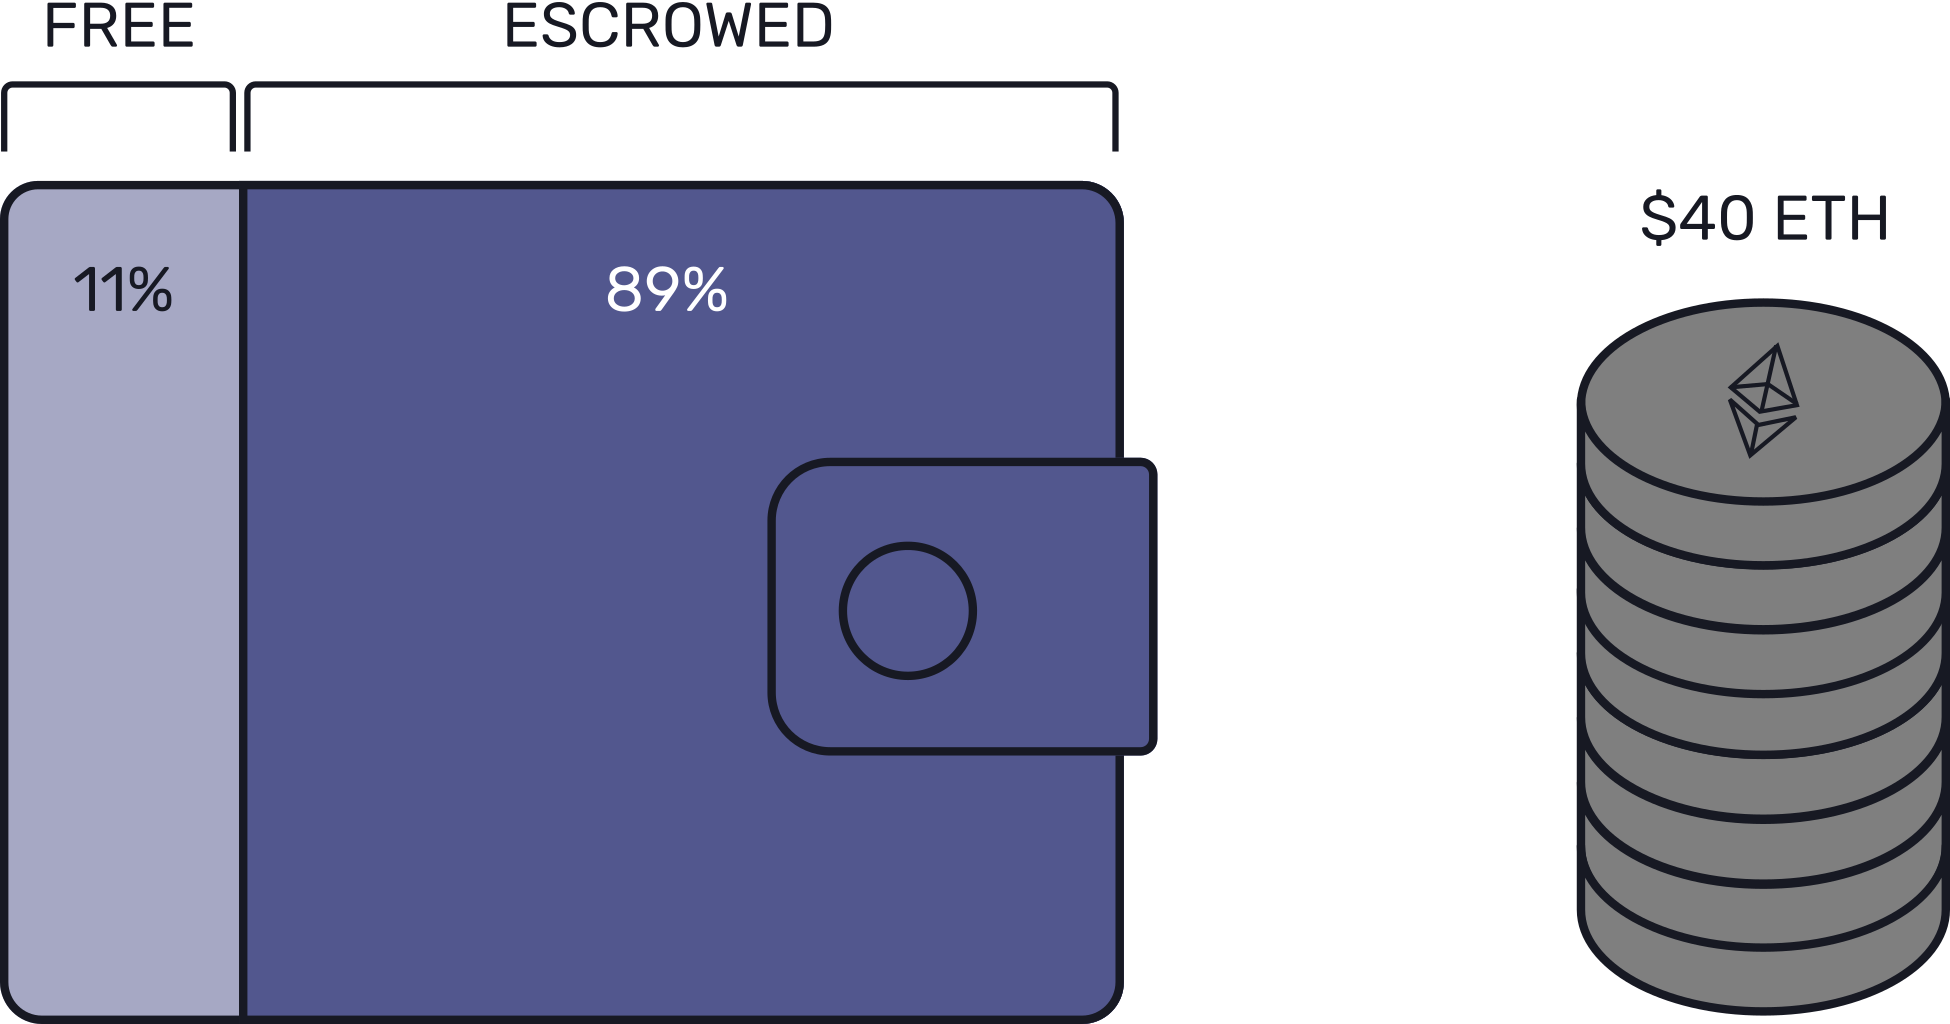
\includegraphics[width=0.6\textwidth]{img/ph_drop}
\end{figure}
\end{enumerate} 

\newpage

\subsection{Fee Evasion}

\noindent Being based on Ethereum, Havven is potentially vulnerable to its tokens being wrapped by another
smart contract which takes deposits, and replicates all exchange functionality on redeemable IOU tokens
it issues. These wrapped tokens could then be exchanged without incurring fees.
\noindent We consider this situation unlikely for a number of reasons. \\

\noindent First, the fees are designed to be low enough that most users
shouldn't notice them, so users will not in general be strongly motivated to switch
to a marginal and less trustworthy alternative. \\

\noindent Second, network effects are tremendously important for currencies; in order to have utility a token must demonstrate acceptability. This is challenging enough in itself, but a wrapped token must do this to an extent that it displaces its own perfect substitute: the token it wraps.
\noindent This would undermine built-in stabilisation mechanisms, which become more powerful with increased transaction volume.Consequently, as a wrapped nomin parasitises more of the nomin market, it destroys the basis of its own utility, which is that nomins themselves are stable. \\

\noindent Finally, it is unlikely that a token wrapper will be credible, not having been publicly and expensively audited, while its primary function undermines the trustworthiness of its authors. \\

\noindent Even so, it's simple to implement a democratic method, weighted by havven balance,
by which havven holders can freeze or confiscate the balance of any contract that wraps assets.
Those havven holders are incentivised not to abuse this system for the same reason that
bitcoin mining pools do not form cartels to double-spend: because abuse of this power
would undermine the value of the system, and thus devalue their own holdings.

\noindent The credible threat of such a system existing is enough to discourage token wrappers
from being used, even if they are written, since any user who does so risks losing their
entire wrapped balance.

\newpage

\subsection{Nomin Demand and Havven Value}

\noindent Being freely-tradable ERC20 tokens, havvens will have a market price which, like
the nomin price, can be measured with an oracle.
Initially, while nomin demand is low, we will use a seven day rolling average of the market price for both havvens and nomins.
This rolling average is designed to smooth out fluctuations in the market price and increase the cost of attacking the system.\\

\noindent However, once nomin transaction volume is sufficiently high, we may instead consider internally estimating
the value of a havven by the fees it is likely to accrue in the future. This value, which implicitly measures nomin volume,
would allow issuance incentives to directly reflect changes in nomin demand.
By using this value instead of the havven market price, the system can avoid the influence of speculation,
since the permitted nomin supply would expand and contract in line with how much nomins are actually being used. \\

\noindent While the system cannot perfectly determine future fee returns and hence nomin demand, it is possible to estimate as a
function of the transaction fees that the system has recently generated.
This computation is designed not to be vulnerable to instantaneous volume spikes, while taking the most recent transaction
volumes to be the most highly-correlated with future volumes:

\vspace{3mm}

\begin{equation}
    V_{t} \approx \sum_{t'=1}^{t} \frac{F_{t - t'}}{(1 + r)^{t'}} \label{eq:price}
\end{equation}

where

\begin{align*} 
& V_{t} \text{: the system's valuation of a havven in period } t  \\
& F_t \text{: the total fees collected in period } t\\
& r \text{: a falloff term}  \\
\end{align*}

\noindent This can be computed efficiently, because $V_{t+1} = \frac{V_t + F_t}{r}$. 
Further, if it is assumed that the average fee take is approximated by $F_t$, and $t$ is large, then:

\vspace{2mm}

\begin{equation}
    V_t \approx \sum_{t'=1}^{\infty} \frac{F_t}{(1 + r)^{t'}} = \frac{F_t}{H \cdot r}
\end{equation}

\vspace{3mm}

\noindent Consequently, $\frac{1}{r}$ approximates the number of periods for a havven to yield a fee return of $V_t$.
A judicious choice of $r$ can then yield a $V_t$ which underestimates the market price of havvens (which also incorporates,
for example, capital gains), while not unduly constraining nomin supply.

\newpage

